\section{Setup and Measurement Procedure}
 We will now explain our experimental setup and then explain what we
 measured.
\subsection{Setup}


There are two scintillators, a NaI scintillator and a PVC
scintillator, see figure \ref{fig:setup}. Each is connected to its
photomultiplier, preamplifier and main amplifier. 
The main amplifiers outputs are connected to delay units and to timing
single channel analyzers (TSCA). The TSCAs are connected
to a coincidence unit. The coincidence unit opens two linear gates, which
connect the TSCAs and multi channel analyzers (MCA). For monitoring purposes we
sometimes connected the coincidence units output to a counter.

\begin{figure}[tbp]
  \centering
  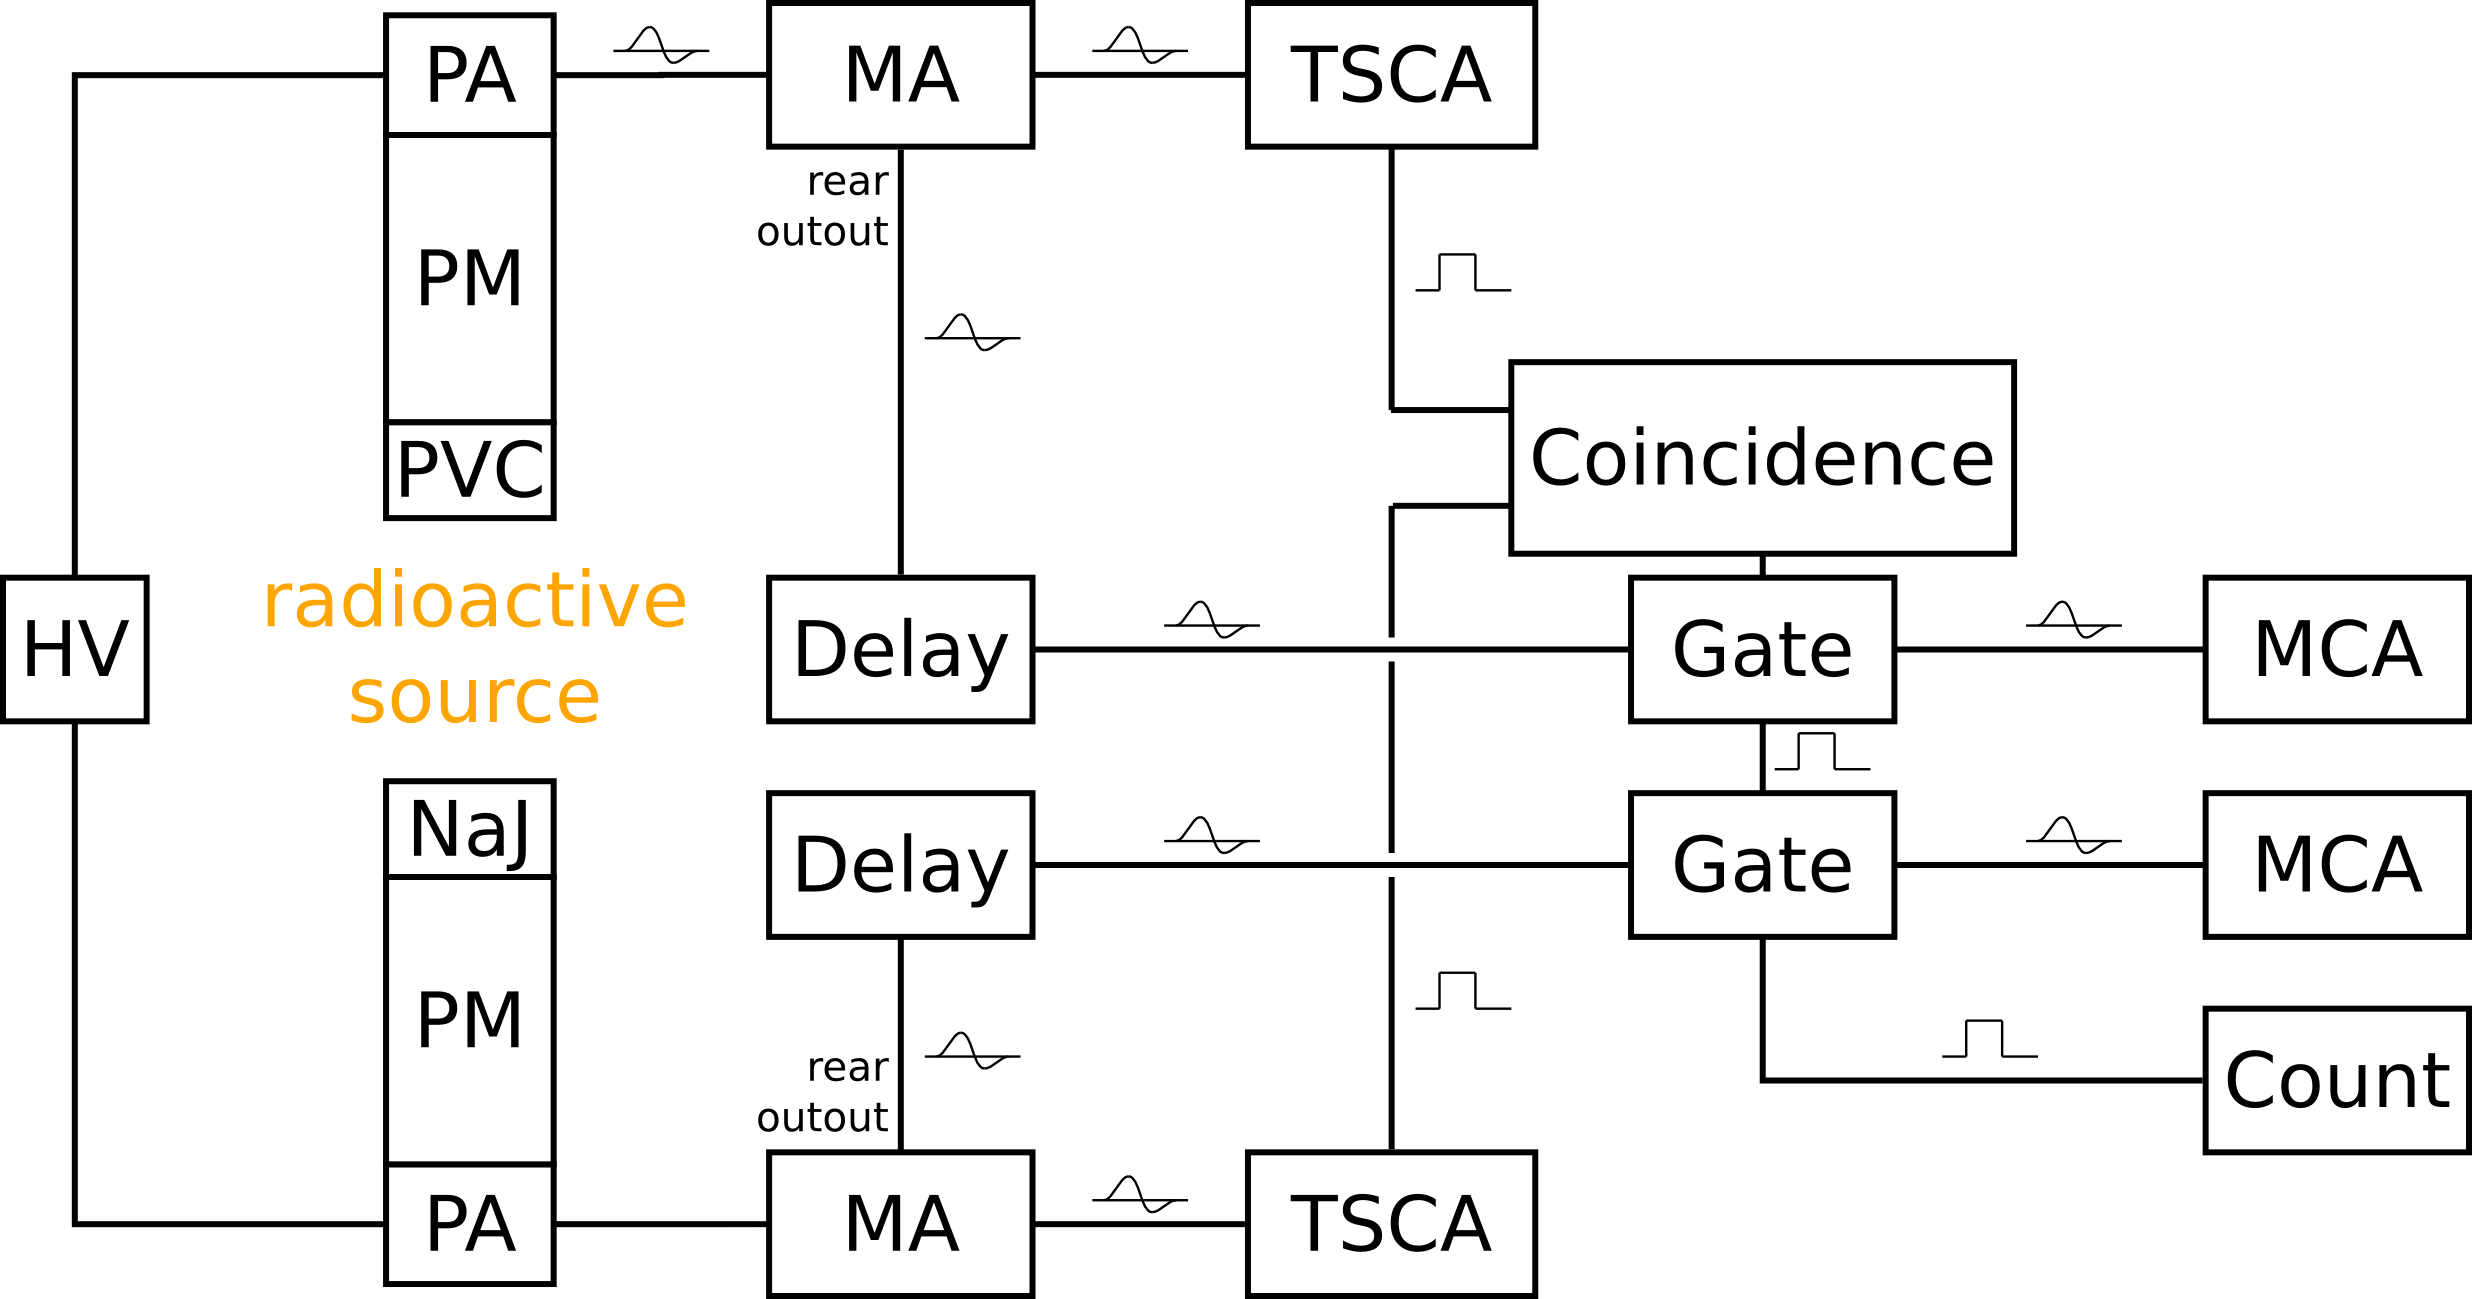
\includegraphics[width=0.9\textwidth]{setup.png}
  \caption{Schematic of our measurement setup.}
  \label{fig:setup}
\end{figure}

%The function of the two scintillators is already explained in the theoretical background, we will now explain shortly the other instruments. In the photomultiplier, the photo-effect takes place, so electrons get free. Those accelerate because of the electric field. When they arrive at a dynode, the electrons knock out other electrons of the dynode. Those accelerate again, and it happens the same at the next dynode. This continues and the number of electrons increases, so in the end the out-coming signal is a higher one. The preamplifier and the main amplifier intensify the incoming signal.


%The delay-unit retards the analogue signal, that is going through the linear gate, which is coming from the main-amplifier. The Timing Single-Channel-Analysator makes the analogue signals into square-wave signals. This unit also can delay the signals. Both units are used to equalize the signals, that they're coming in at once.  The coincidence unit overlies the square-wave-signals, as long as they're contemporary the linear gate opens. There are two linear gates, one is obstructed with the coincidence unit the other one is external. The linear gate is as long open, as the signals are coincidence, if at the same time  the signal of the delay unit is coming in too, an analogue signal is coming out.  The multichannel-analyzer distributes the amplitudes to channels, what enables processing the data with the computer.


The TSCAs convert the analogous pulses into digital ones, if the pulse height is
inside certain limits, called windows. These digital pulses can be delayed.
The coincidence unit checks the simultaneity of the signals from both
TSCAs. 
%Two incoming $\gamma$-quanta are simultaneous, if they arrive in a short time, the timing resolution of the coincidence unit. 
To ensure that the signals of two simultaneous registered events are arrive
at the same time in the coincidence unit, one must consider
that the cables have the same length. For that we observed our signals at
the oscilloscope and adjusted delays so that the signals were
coincidence.
If the two digital pulses arrive at the same time, the coincidence unit
opens the two linear gates (one internal and one external). The analogues
signals from two simultaneously registered events are then processed by the
multichannel analyzer. The multichannel analyzer is an impulse level
analyzer. He distributes the
impulses, depending on their voltage level, to different channels.
This setup allows us to measure the spectrum of coincident events only. In
our case the scattered electron in the PVC scintillator and the scattered
photon in the NaI scintillator are detected at the same time. 


\subsection{Measurement Procedure}

\subsubsection{Delay Setting}
First of all we arranged the setup with all devices and adjusted the delays
for the scintillators. To do this, we placed the \Na  source in the center
of both scintillators to compare all the signals (TSCA outputs and analogous
delayed signals) with the
oscilloscope. The annihilation photons from the beta decay are detected
simultaneously. This allows us to set the delays. The two digital TSCA
signals must arrive at the same time to
trigger the coincidence unit, and the two analogous delayed signals must
arrive when the two linear gates are open. Our settings are in the appendix,
table \ref{tab:delays} and \ref{tab:amps}. It is
important to set the delays with all devices implemented before making the
energy calibration. If the
delay and coincidence equipment had been installed after the energy
calibration, the calibration would be void, because the additional
equipment alters the analogous signal what results in energy shifts in later
measurements.

\subsubsection{Energy Calibration}
Before starting our measurement we made the energy calibration. For that we
record the direct $\gamma$ spectrum of \Na and \Cs with both scintillators. 
The energy of characteristic peaks in these spectra are known, what allows
us to gauge the channel axis.

\subsubsection{Conservation of Energy and Differential Cross Section}
For different scattering angles $\theta$ we recorded the electron (PVC) and
photon spectrum (NaI) for coincident events produced by \compton scattering
in the PVC scintillator. The radiation source is \Cs. This allows us to test
the conservation of energy. We have measured for $\theta =0\degree$ through
$120\degree$ in $15\degree$ steps. The measurement duration was
$t=3600\mathrm{s}$ each.

The last part was to measure the differential cross section and to compare
it with
the \kleinn  formula. We can use the data from the previous measurement to
determine the scattered photon intensities. To determine the primary photon
intensity, i.e. the intensity of the unshielded \Cs source, we have measured
the \Cs source (without the PVC scintillator blocking the radiation) with
the NaI scintillator for $t=3600\mathrm{s}$.

\subsubsection{Background an Random Coincidence}
Over the nights we measured the background and random coincidence. To
measure the background with each scintillator separately we turned the
\Cs  source sideways. For the random coincidence we added additional
delay to the NaI signals ($4\mu \mathrm{s}$ for digital TSCA output and
analogous signal). This causes coincident events not to trigger the coincident
unit. We have used the cesium source. 

